\chapter{Representación Gráfica de la Suma}
\section{Suma}
La suma de vectores puede representarse de manera gr\'afica, respetando las siguientes propiedades.

\subsection{Propiedades de la Suma}
\begin{itemize}
    \item Conmutatividad: $\vec{A} + \vec{B} = \vec{B} + \vec{A}$
    \item No conmutativa para la resta: $\vec{A} - \vec{B} \neq \vec{B} - \vec{A}$
    \item Relaci\'on: $\vec{A} - \vec{B} = \vec{A} + (-\vec{B}) = -\vec{B} + \vec{A}$
\end{itemize}

\subsection{Suma de Dos Vectores}

\begin{center}
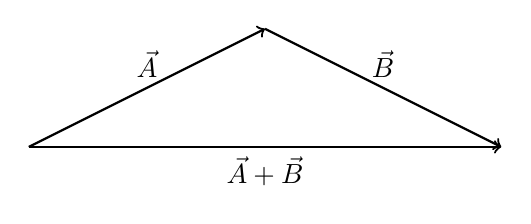
\begin{tikzpicture}[scale=1.5]
    % Vector A
    \draw[->, thick] (0,0) -- (2,1) node[midway, above] {$\vec{A}$};
    % Vector B
    \draw[->, thick] (2,1) -- (4,0) node[midway, above] {$\vec{B}$};
    % Resultante A + B
    \draw[->, thick] (0,0) -- (4,0) node[midway, below] {$\vec{A} + \vec{B}$};
\end{tikzpicture}
\end{center}


\subsection{Suma de Tres Vectores}

\begin{center}
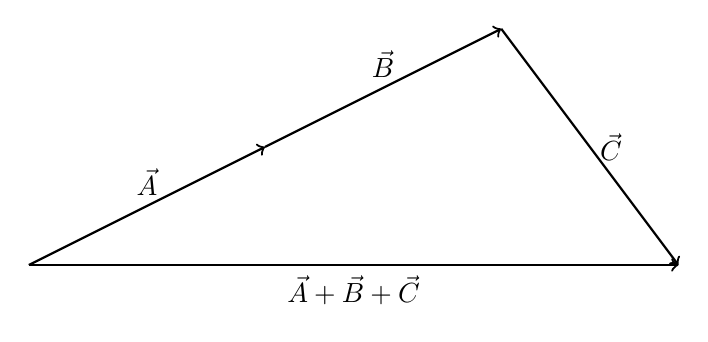
\begin{tikzpicture}[scale=1.5]
    % Vector A
    \draw[->, thick] (0,0) -- (2,1) node[midway, above] {$\vec{A}$};
    % Vector B desde el final de A
    \draw[->, thick] (2,1) -- (4,2) node[midway, above] {$\vec{B}$};
    % Vector C desde el final de B
    \draw[->, thick] (4,2) -- (5.5,0) node[midway, right] {$\vec{C}$};
    % Resultante A + B + C
    \draw[->, thick] (0,0) -- (5.5,0) node[midway, below] {$\vec{A} + \vec{B} + \vec{C}$};
\end{tikzpicture}
\end{center}

 \newpage
\section{Resta de Vectores}
La resta de vectores puede representarse como la suma de un vector con el opuesto de otro.

\begin{center}
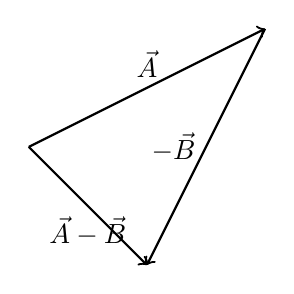
\begin{tikzpicture}[scale=1.5]
    % Vector A
    \draw[->, thick] (0,0) -- (2,1) node[midway, above] {$\vec{A}$};
    % Vector -B desde el final de A
    \draw[->, thick] (2,1) -- (1,-1) node[midway, left] {$-\vec{B}$};
    % Resultante A - B
    \draw[->, thick] (0,0) -- (1,-1) node[midway, below] {$\vec{A} - \vec{B}$};
\end{tikzpicture}
\end{center}
\section{Desplazamientos Utilizando Puntos Cardinales}

\subsection{Sistema de Puntos Cardinales}

\begin{center}
\begin{tikzpicture}[scale=1.5]
    % Ejes cardinales
    \draw[->, thick] (0,0) -- (0,2) node[above] {N};
    \draw[->, thick] (0,0) -- (2,0) node[right] {E};
    \draw[->, thick] (0,0) -- (0,-2) node[below] {S};
    \draw[->, thick] (0,0) -- (-2,0) node[left] {O};
\end{tikzpicture}
\end{center}
\subsection{Desplazamiento en una Direcci\'on Espec\'ifica}

Un desplazamiento de $30^{\circ}$ hacia el norte del este se puede representar gr\'aficamente como sigue:

\begin{center}
\begin{tikzpicture}[scale=1.5]
    % Ejes cardinales
    \draw[->, thick] (0,0) -- (0,2) node[above] {N};
    \draw[->, thick] (0,0) -- (2,0) node[right] {E};
    \draw[->, thick] (0,0) -- (0,-2) node[below] {S};
    \draw[->, thick] (0,0) -- (-2,0) node[left] {O};
    % Direcci\'on
    \draw[->, thick] (0,0) -- (1.73,1) node[midway, above right] {};
    % Angulo
    \draw[thick] (1,0) arc[start angle=0, end angle=30, radius=1cm];
    \node at (1.3,0.2) {$30^{\circ}$};
\end{tikzpicture}
\end{center}

\subsection{Rotaci\'on}

La notaci\'on del desplazamiento es:

\begin{itemize}
    \item Rotaci\'on: \textbf{E $30^{\circ}$ N}
\end{itemize}

\section*{Representación gráfica de desplazamientos}

\subsection*{Gráfico inicial}

\begin{center}
\begin{tikzpicture}
  % Ejes cardinales
  \draw[->] (0,-2.5) -- (0,2.5) node[above] {N};
  \draw[->] (-2.5,0) -- (2.5,0) node[right] {E};
  \node[below] at (0,-2.5) {S};
  \node[left] at (-2.5,0) {O};

  % Primer vector (30° este del norte)
  \draw[->,thick] (0,0) -- (1.5,2) node[midway, above right] {$30^\circ$};
  \draw[dashed] (0,0) -- (0,2);
  \node[above right] at (0.5,1) {E $30^\circ$ N};
\end{tikzpicture}
\end{center}

\subsection{Ejemplo de aplicación}

\textbf{Enunciado:} Un excursionista sale de su base y se desplaza:
\begin{itemize}
  \item $7\,\mathrm{km}$ en dirección $20^\circ$ este del norte.
  \item Luego, $10\,\mathrm{km}$ en dirección $40^\circ$ este del norte.
  \item Finalmente, $15\,\mathrm{km}$ hacia el suroeste.
\end{itemize}

\textbf{Determinaciones:}
\begin{enumerate}
  \item Haga un esquema vectorial de los tres desplazamientos.
  \item Escriba cada vector desplazamiento en componentes de un sistema de coordenadas rectangulares.
  \item Determine el desplazamiento total del excursionista.
  \item Si tuviera que regresar directamente a su base, ¿qué distancia recorrería y qué dirección debería tomar?
\end{enumerate}

\section{Diagrama de Cuerpo Libre y Segunda Ley de Newton}

\subsection*{Diagrama de Cuerpo Libre (DCL)}
El diagrama de cuerpo libre (DCL) es la representación de todas las fuerzas que actúan sobre un objeto.

\subsection*{Gráfico del DCL}

\begin{center}
\begin{tikzpicture}[scale=1.5,>=stealth]

    % Ejes principales
    \draw[->] (0,0) -- (2,0) node[below right] {$\vec{F}_2$};
    \draw[->] (0,0) -- (0,2) node[above left] {$\vec{F}_1$};
    \draw[->] (0,0) -- (-1.5,-1.5) node[below left] {$\vec{F}_3$};
    \draw[->] (0,0) -- (1,-2) node[below right] {$\vec{F}_4$};

    % Nodo central
    \filldraw (0,0) circle (2pt) node[below left] {V};

    % Etiquetas de las fuerzas
    \node at (1.5,0.1) {$\vec{F}_2$};
    \node at (0.1,1.5) {$\vec{F}_1$};
    \node at (-1.1,-1.2) {$\vec{F}_3$};
    \node at (0.8,-1.7) {$\vec{F}_4$};

\end{tikzpicture}
\end{center}

\subsection*{Fuerzas Actuantes}
Existen 4 fuerzas actuando sobre un objeto, en la dirección indicada por las flechas.

\subsection*{Segunda Ley de Newton}
La segunda ley de Newton nos entrega la información de la aceleración del objeto cuando este está sometido a varias fuerzas que actúan simultáneamente.


\section{Representación de Vectores y Segunda Ley de Newton}

\subsection{1. Representación Matemática}
Siempre los vectores se escriben en base de coordenadas. Matemáticamente, la segunda ley de Newton se expresa como:

\[
\sum \vec{F} = m\vec{a} \quad \rightarrow \quad 
\begin{cases}
\sum F_x = m a_x \\
\sum F_y = m a_y
\end{cases}
\]

\section{Cálculo de componentes de las fuerzas}
Ejemplo: Tres fuerzas actúan simultáneamente sobre un objeto de masa \(2 \, \mathrm{kg}\).  
Las fuerzas se indican en la figura:

\begin{center}
    \begin{tikzpicture}[scale=1.5,>=stealth]
        % Ejes coordenados
        \draw[->] (-2.5,0) -- (2.5,0) node[right] {$x$};
        \draw[->] (0,-2.5) -- (0,2.5) node[above] {$y$};

        % Nodo principal
        \filldraw (0,0) circle (1.5pt) node[below right] {};

        % Vectores
        \draw[->,thick] (0,0) -- (2,1.15) node[midway, above right] {$\vec{F}_1 = 10 \, \mathrm{N}$};
        \draw[->,thick] (0,0) -- (-2,0) node[midway, below] {$\vec{F}_2 = 15 \, \mathrm{N}$};
        \draw[->,thick] (0,0) -- (1,-1.5) node[midway, right] {$\vec{F}_3 = 8 \, \mathrm{N}$};

        % Ángulos
        % Ángulo de F1 con eje x positivo
        \draw[->] (0.5,0) arc[start angle=0,end angle=30,radius=0.5];
        \node at (0.6,0.3) {$30^\circ$};

        % Ángulo de F3 con eje negativo y
        \draw[->] (0.3,-0.3) arc[start angle=270,end angle=230,radius=0.5];
        \node at (0.5,-0.6) {$40^\circ$};

        % Líneas auxiliares para ángulos
        \draw[dashed] (2,1.15) -- (2,0);
        \draw[dashed] (1,-1.5) -- (1,0);
    \end{tikzpicture}
\end{center}
Calcular las componentes de la aceleración del objeto.

\newpage
\section{Aplicacion de la segunda ley de Newton}
\section*{Aplicación de la 2\textsuperscript{a} ley de Newton a un Diagrama de Cuerpo Libre (DCL)}

Todos estos fuerzas están actuando simultáneamente según la \textbf{segunda ley de Newton}:

\[
\sum \vec{F} = m\vec{a}
\]

\begin{center}
    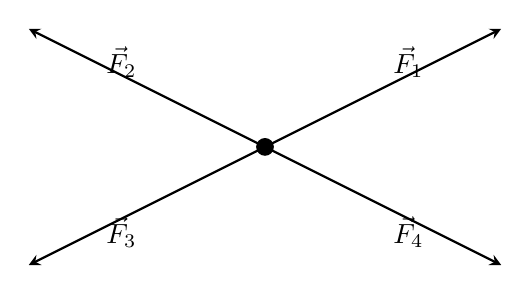
\begin{tikzpicture}[scale=1.5,>=stealth]
        % Nodo central
        \filldraw (0,0) circle (2pt);

        % Flechas de fuerzas
        \draw[->,thick] (0,0) -- (2,1) node[midway, above right] {$\vec{F}_1$};
        \draw[->,thick] (0,0) -- (2,-1) node[midway, below right] {$\vec{F}_4$};
        \draw[->,thick] (0,0) -- (-2,1) node[midway, above left] {$\vec{F}_2$};
        \draw[->,thick] (0,0) -- (-2,-1) node[midway, below left] {$\vec{F}_3$};

        % Etiquetas en las flechas
        \node at (0,0) [below right] {};
    \end{tikzpicture}
\end{center}
\vspace{0.5cm}
\textit{Segunda Ley de Newton:} Cuando varias fuerzas actúan sobre un objeto, la fuerza neta es igual a la masa multiplicada por la aceleración.

\section{solucionario}
Los componentes de la aceleración del objeto los veremos a continuación : 

\section*{Cálculo de $a_x$ y $a_y$}

\textbf{Solución:}

Aplicamos la \textbf{2\textsuperscript{a} ley de Newton}:

\[
\sum F_x = ma_x \implies 10 \cos 30^\circ - 15 + 8 \cos 40^\circ = 2 \cdot a_x
\]

De lo anterior, se tiene:

\[
a_x = \frac{10 \cos 30^\circ - 15 + 8 \cos 40^\circ}{2} \approx 0.11 \, \mathrm{m/s^2}
\]


\section{Unidades del Sistema Internacional (S.I.)}

\[
[\vec{F}] = \mathrm{N}, \quad [m] = \mathrm{Kg}, \quad [\vec{a}] = \mathrm{m/s^2}
\]

Aplicando la \textbf{2\textsuperscript{a} ley de Newton}:

\[
\sum F_y = ma_y \implies 10 \sin 30^\circ - 8 \sin 40^\circ = 2 \cdot a_y
\]

De lo anterior, se tiene:

\[
a_y = \frac{10 \sin 30^\circ - 8 \sin 40^\circ}{2}
\]

Resolviendo:

\[
a_y = 5 \sin 30^\circ - 4 \sin 40^\circ \approx -0.07 \, \mathrm{m/s^2}
\]

Finalmente, el vector aceleración es:

\[
\vec{a} \approx -0.11\hat{i} - 0.07\hat{j} \, \mathrm{m/s^2}
\]
\section{Equilibrio}
\[
\sum \vec{F} = 0
\]
\subsection*{Aplicación}

\[
\sum F_x = 0 \quad \text{y} \quad \sum F_y = 0
\]

\begin{center}
\begin{tikzpicture}[scale=1.5]
    % Nodo central
    \draw[fill=black] (0,0) circle (1pt);
    
    % Vectores
    \draw[->, thick] (0,0) -- (2,0.5) node[midway, above right] {$\vec{F}_1$};
    \draw[->, thick] (0,0) -- (-1.5,-1.5) node[midway, left] {$\vec{F}_2$};
    \draw[->, thick] (0,0) -- (-1,1.5) node[midway, left] {$\vec{F}_3$};
    
    % Arcos
    \draw[thick] (1,0) arc[start angle=0, end angle=15, radius=1cm];
    \node at (1.2,0.2) {$\theta$};
\end{tikzpicture}
\end{center}
